\subsection{802.11 Data Transmission}
\label{subsec:tx}

In this section, we first show that our
verification framework can improve verification precision by inferring
the missing or extra packets using the augmented transition
framework. We then demonstrate the ability of our framework to detect true violations by
manually introducing bugs in the \ns{} implementation and show the precision and
recall of validation results.


\begin{comment}
\begin{figure*}[t!]
  \centering
  \begin{subfigure}{0.33\textwidth}
    \centering
    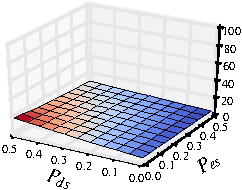
\includegraphics[width=\textwidth]{./figures/scripts/StepCount3DFigure_0_10.pdf}
    \caption{$Pr_{ed} \in [0.05, 0.10, 0.15]$}
  \end{subfigure}\hspace*{0.01\textwidth}
  \begin{subfigure}{0.33\textwidth}
    \centering
    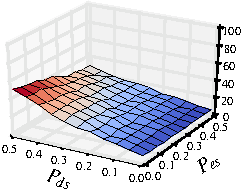
\includegraphics[width=\textwidth]{./figures/scripts/StepCount3DFigure_0_30.pdf}
    \caption{$Pr_{ed} \in [0.20, 0.25, 0.30, 0.35]$}
  \end{subfigure}\hspace*{0.01\textwidth}
  \begin{subfigure}{0.33\textwidth}
    \centering
    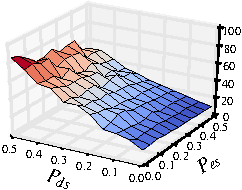
\includegraphics[width=\textwidth]{./figures/scripts/StepCount3DFigure_0_50.pdf}
    \caption{$Pr_{ed} \in [0.40, 0.45, 0.50]$}
  \end{subfigure}\hspace*{0.01\textwidth}
  \caption{\textbf{Average Searching Step Per Packet.} For each data point, the mean of 5 runs
  is used.}
  \label{fig:cost}
\end{figure*}
\end{comment}


\vspace*{-3mm}
\subsubsection{Experimental Setup}

We set up two \wifi{} devices acting as the transmitter (DUT) and receiver
respectively. Another \wifi{} device is configured in monitor mode and acts as
the sniffer. During the experiments,we collect both the DUT packet trace
(the ground truth) and the sniffer trace.

\vspace*{-3mm}
\subsubsection{Verifying Unmodified Implementation}

In the original monitor state machine shown in Fig.~\ref{fig:dot11_tx_ta}, we
set acknowledgment timeout $T_o=334\mu$s, maximum retransmission delay
$T_m=15$ms according to the protocol. We also adapt the state machine to include
multiple retransmissions\footnote{The exact number of retransmissions is not
part of the protocol, and NS-3 implementation set this to be 7.} instead of one.

Let $Pr_{ds}$, $Pr_{es}$ and $Pr_{ed}$ be the packet loss probability between
the DUT and sniffer, endpoint and sniffer, DUT and endpoint respectively.
$Pr_{ed}$ represents the characteristics of the system being tested, while
$Pr_{ds}$ and $Pr_{es}$ represent the sniffer's quality in capturing packets.



We vary each of the three probability, $Pr_{ds}$, $Pr_{es}$ and $Pr_{ed}$, from
0 to 0.5 (both inclusive) with 0.05 step.  For each loss ratio combination, we
ran the experiment 5 times, and each run lasted
30 seconds. In total, 6655 ($11^3\times 5$) pair of DUT and sniffer packet
traces were collected.

To establish the ground truth of violations, we first verify the DUT packet
traces using the \textit{original} state machine $S$.  This can be achieved by
disabling augmented transitions in our framework.  As expected, no violation is
detected in any DUT packet traces.

We then verify the sniffer traces using the augmented state machine $S^+$.  For
the $\mathit{GoBack}(k)$ heuristic, we set $k=7$, which is the maximum number of
transmissions of a single packet. For the $\mathit{NumMissing}(d, l, k)$ heuristic, we
set the sliding window size $l=100$, and $k=80$ such that no violation is
reported. The relationship of $k$ and validation precision is studied in next
section.

Next, we present detailed analysis of the augmented transitions on the sniffer
traces. The goal is to study for a given system packet loss probability
$Pr_{ed}$, how the sniffer packet loss properties ($Pr_{ds}$ and $Pr_{es}$)
affect the difference between the DUT trace and the mutation trace, which represents
a guess of the DUT trace by the augmented state machine based on the sniffer
trace.

For all following analysis, we divide the traces into three groups according to
$Pr_{ed}$: low ($0 \le Pr_{ed} \le 0.15$), medium ($0.20 \le Pr_{ed} \le 0.35$)
and high ($0.40 \le Pr_{ed} \le 0.50$).

\begin{comment}
Fig.~\ref{fig:consec_aug} shows the distribution of Maximum Consecutive
Augmented Transitions (MCAT) in the mutation trace. First, for a given system
loss ratio $Pr_{ed}$, the higher the sniffer packet loss probability, the larger
the MCAT. In particular, the MCAT peaks when the sniffer missed 50\% packets both
from the DUT and the EP. Second, when the system loss ratio gets higher, the
peak of MCAT decreases. This is due to the fact that the ratio of retransmission
packets increases when $Pr_{ed}$ gets higher. Since all the retransmission
packets with the same sequence number are identical, the uncertainty can be
resolved with potentially fewer retransmission packets than what the DUT
actually sent. In other words, the major uncertainty is the \textit{existence},
nor the \textit{number} of retransmission packets.
\end{comment}

The different between two packet traces can be quantified by the Jaccard distance
metric.%
\begin{align}
  Jaccard(Tr_1, Tr_2) = \frac{Tr_1 \ominus Tr_2}{Tr_1 \cup Tr_2}
\end{align}%
where $\ominus$ is the symmetric difference operator.
The distance is 0 if the
two traces are identical, and is 1 when the two traces are completely different.
The smaller the distance is, the more similar the two traces are.

\begin{comment}
A naive way to calculate the distance is to use the hash the $(t, p)$ pair for
set intersection and union operation.
However, it does not work for mutation
trace which contains fabricated packets with no actual payload.
Therefore, we use
a protocol specific canonical representation of packets when calculating the
distance.
In particular, the string \texttt{r\_DATA\_i\_t} represents the $t^{th}$
transmission of a data packet with sequence number $i$.
$r$ represents the round
of sequence numbers as it wraps after 4096.
And similarly \texttt{r\_Ack\_i\_t} is the corresponding acknowledgment packet.
\end{comment}

\begin{figure*}[t!]
  \centering
  \begin{subfigure}{0.33\textwidth}
    \centering
    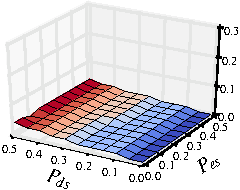
\includegraphics[width=\textwidth]{./figures/scripts/MutationDUTJaccard3DFigure_0_10.pdf}
    % \caption{$Pr_{ed} \in [0.05, 0.1, 0.15]$}
    \caption{$0.05 \le Pr_{ed} \le 0.15$}
  \end{subfigure}\hspace*{0.01\textwidth}
  \begin{subfigure}{0.33\textwidth}
    \centering
    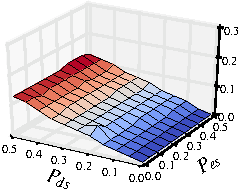
\includegraphics[width=\textwidth]{./figures/scripts/MutationDUTJaccard3DFigure_0_30.pdf}
    \caption{$0.2 \le Pr_{ed} \le 0.35$}
  \end{subfigure}\hspace*{0.01\textwidth}
  \begin{subfigure}{0.33\textwidth}
    \centering
    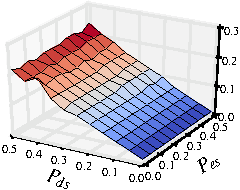
\includegraphics[width=\textwidth]{./figures/scripts/MutationDUTJaccard3DFigure_0_50.pdf}
    \caption{$0.4 \le Pr_{ed} \le 0.5$}
  \end{subfigure}\hspace*{0.01\textwidth}
  \caption{\textbf{Jaccard Distance Between Mutation and DUT Traces.} For each
  data point, the mean of the 5 runs is used.}
  \label{fig:mutation_dut}
  \vspace*{-5mm}
\end{figure*}


Fig.~\ref{fig:mutation_dut} shows the Jaccard Distance between mutation and its
corresponding DUT trace. We make the following observations. First, for a given
system loss probability $Pr_{ed}$ (each sub-figure), the lower the sniffer
packet loss probability ($Pr_{ds}$ and $Pr_{es}$), the smaller Jaccard distance
between the DUT and mutation trace. Intuitively, this means a sniffer that
misses less packets can enable our framework to better reconstruct the DUT
trace.

Second, we observe a \textit{protocol-specific} trend that $Pr_{ds}$ is more
dominant than $Pr_{es}$.  This is because retransmission packets of the same
sequence number are identical, hence when the sniffer misses multiple
retransmission packets, our framework only needs to infer one retransmission
packet to continue state machine execution.

Finally, as the system loss probability $Pr_{ed}$ increases, the Jaccard
distance increases more rapidly as $Pr_{ds}$ increases.  This is because the
ratio of retransmission packet increases along with $Pr_{ed}$.


\begin{comment}

Finally, We evaluate the cost of resolving uncertainty. In particular, we use
the Average Search Steps Per Packet (ASSPP) as a metric to quantify the search
cost.  It is calculated by dividing the total number of search steps by the
number of packets in the packet trace. For DUT traces, ASSPP is always 1 since
there is not uncertainty. For sniffer traces, however, multiple search steps has
be to conducted to resolve the potential uncertainty of each packet in the
sniffer trace.



Fig.~\ref{fig:cost} shows the distribution of ASSPP at different $Pr_{ed}$.
Similar to the case in Fig.~\ref{fig:mutation_dut}, $Pr_{ds}$ plays a dominant
role in determine the searching cost. One interesting observation is that the
search cost peaks when $Pr_{ds}$ is high while $Pr_{es}$ is low. In such loss
probability combinations, sniffer misses many data packets from the DUT but
picks up lots of \textit{dangling} $Ack$ packets from the EP. Because the $Ack$
packet has neither sequence numbers nor retry flag, the searching algorithm had
a hard time resolving such uncertainty.
\end{comment}

\vspace*{-3mm}
\subsubsection{Introducing Bugs}

We have demonstrated that our framework can tolerate sniffer imperfection and
avoid raising false alarms.  The next question is, can it detect true
violations?  To answer this question, we manually introduce several bugs in
\ns{} implementation that concerns various aspects of 802.11 data transmission
protocol.  More specifically, the bugs are:

\begin{itemize}
  \item \textbf{Sequence Number}\quad The DUT does not assign sequence number
    correctly. For example, it may increase sequence by 2 instead of 1, or it
    does not increase sequence number after certain packet, etc. We choose one
    type of such bugs in each run.
  \item \textbf{Semantic}\quad The DUT may retransmit even
    after receiving $Ack$, or does not retransmit when not receiving $Ack$.
\end{itemize}

We instrument the \ns{} implementation to embed instances of bugs in each
category. At each experiment run, we randomly decide whether and which bug to
introduce for each category. We fix $Pr_{ds}=Pr_{es}=0.1$ and vary $Pr_{ed}$
from 0.0 to 0.5 with 0.01 step. For each $Pr_{ed}$ value, we ran the experiment
100 times, of which roughly 75 experiments contained bugs. In total, 5100 pairs of
DUT and sniffer traces were collected.


We use the DUT packet traces as ground truth of whether or not each experiment
run contains bugs.
For each $Pr_{ed}$ value, we calculate the precision and recall of violation
detection using the sniffer traces.%
\begin{align}
  \text{Precision} = \frac{\{\text{Reported Bugs}\} \cap \{\text{True Bugs}\}}{\{\text{Reported Bugs}\}}\\
  \text{Recall} = \frac{\{\text{Reported Bugs}\} \cap \{\text{True Bugs}\}}{\{\text{True Bugs}\}}
\end{align}%
The precision metric quantifies how \textit{useful} the validation results are ,
while the recall metric measures how \textit{complete} the validation results
are.

\begin{figure}[t!]
  \centering
  \begin{subfigure}{0.48\textwidth}
    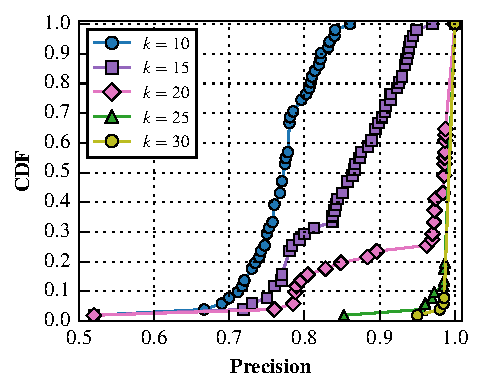
\includegraphics[width=\textwidth]{./figures/scripts/PrecisionFigure.pdf}
  \end{subfigure}
  \begin{subfigure}{0.48\textwidth}
    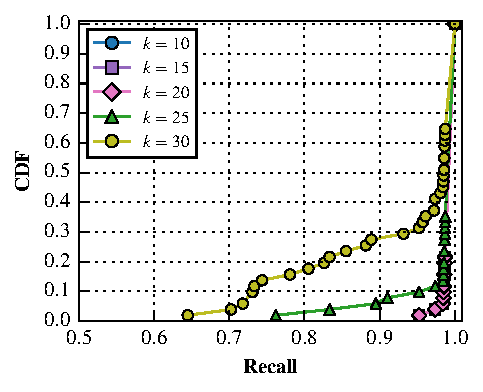
\includegraphics[width=\textwidth]{./figures/scripts/RecallFigure.pdf}
  \end{subfigure}
  \caption{\textbf{Precision and Recall of Validation Results.}}
  \label{fig:precision}
  \vspace*{-5mm}
\end{figure}

Fig.~\ref{fig:precision} shows the CDF of precision and recall of the 51
experiments for various $k$ values. For precision, as expected, the more
tolerant the search to sniffer losses (larger $k$), the more tolerant the
framework is to sniffer losses, and the more precise the violation detection. In
particular, when $k=30$, the precisions are 100\% for all $Pr_{ed}$ values.
Second, the recall is less sensitive to the choice of $k$.  Except for the
extreme case when $k=30$, all other thresholds can report almost all the
violations.
